\documentclass[a4paper, 11pt]{article}
\usepackage{color}
\usepackage{fancyhdr}
\usepackage{float}
\usepackage{stfloats}
\usepackage{placeins}
\usepackage{tabularray}
\usepackage{xcolor,colortbl}
\usepackage[top=2.5cm, bottom=2cm, left = 2.5cm, right = 2.5cm]{geometry} 
\geometry{a4paper} 
\usepackage[utf8]{inputenc}
\usepackage{textcomp}
\usepackage{graphicx} 
\usepackage{amsmath,amssymb}  
\usepackage{bm}  
\usepackage[pdftex,bookmarks,colorlinks,breaklinks]{hyperref} 
\hypersetup{linkcolor=MSBlue,citecolor=black,filecolor=black,urlcolor=black} % black links, for printed output
\usepackage{memhfixc} 
\usepackage{pdfsync}  
\usepackage{xcolor}
\usepackage{titlesec}
\usepackage{tocloft}
\usepackage{rotating}

\definecolor{MSBlue}{RGB}{47, 84, 150}
\definecolor{MSGray}{RGB}{128, 128, 128}

\renewcommand{\cftsecfont}{\fontfamily{qag}\selectfont\bfseries} 
\renewcommand{\cftsecpagefont}{\fontfamily{qag}\selectfont\bfseries\color{MSBlue}} 
\renewcommand{\cfttoctitlefont}{\fontfamily{qag}\selectfont\LARGE\bfseries}               
\renewcommand{\familydefault}{phv}

\fancypagestyle{titlepage}{
  \fancyhf{}
  \rfoot{\fontfamily{qag}\fontsize{11pt}{0pt}\selectfont\color{MSGray} version 0.2v}
  \renewcommand{\headrulewidth}{0pt}
  \renewcommand\footrulewidth{0pt}
}



\pagestyle{fancy}
\renewcommand{\headrulewidth}{0pt}
\renewcommand{\footrulewidth}{0pt}
\setlength{\headheight}{15pt}
\rhead{\fontfamily{qag}\fontsize{10pt}{12pt}\selectfont\color{MSGray} 05.06.23}
\lhead[]{}
\fancyfoot[C]{\fontsize{10pt}{10pt}\selectfont\thepage} 



\titleformat{\section}
  {\fontfamily{qag}\selectfont\LARGE\bfseries\color{MSBlue}}
  {\thesection}{0.5em}{}
  
  
\titleformat{\subsection}
  {\fontfamily{qag}\selectfont\Large\mdseries\color{MSBlue}}
  {\thesubsection}{0.5em}{}

\titleformat{\subsubsection}
  {\fontfamily{qag}\selectfont\large\mdseries\color{MSBlue}}
  {\thesubsubsection}{0.5em}{}

\titlespacing\subsubsection{0pt}{12pt plus 4pt minus 2pt}{0pt plus 2pt minus 2pt}

\linespread{1.2} 

\begin{document}

\begin{titlepage}
  \thispagestyle{titlepage}
  \begin{center} 
    
\includegraphics[width=200pt]{qs.png}
    \end{center}


	\setlength{\parindent}{0pt}
	\vspace*{.15\textheight}
	\medbreak
	{\fontfamily{qag}\Huge\bfseries\color{MSBlue}CanvasDataMicroservice Report\par}
	\bigbreak
    \bigbreak
	{Michał Raczkowski\par}
    \smallbreak
    {\small OL S6 \par}
    \smallbreak
    {\small 4465024\par}
\end{titlepage}



\pagebreak


\tableofcontents

\vfill
\begin{table}[b]
  \centering
  \begin{tblr}{
    width = \linewidth,
    colspec = {Q[200]Q[133]Q[327]Q[248]},
    hlines,
    vlines,
  }
  \textbf{Version} & \textbf{Date} & \textbf{Author} & \textbf{Comment} \\
   0.1v                & 04.06.23             & M. Raczkowski   & Overview,Design,Data processing, Conclusion \\
   0.2v    & 05.06.23 & M. Raczkowski, G. Malisz & Clean up and edit, Optimalisation

  \end{tblr}
\end{table}


\pagebreak


\section{Overview}
The Canvas Data Microservice collects data on student scores, submissions, and grades from the Canvas learning management system. It organizes and stores this data for analysis. The Analyze Microservice processes the collected data. These insights are then presented in a web application dashboard, providing users with a user-friendly interface to visualize and explore the data. The dashboard allows administrators, instructors, and students to make data-driven decisions to improve educational outcomes.

\section{Design}


\subsection{Domain-Driven Design}
The Canvas Data Microservice is designed following the principles of Domain-Driven Design (DDD), offering significant advantages to the overall software structure. By embracing DDD, the microservice ensures a cohesive and maintainable system. It focuses on a clear domain model, identifying key concepts and entities of the educational domain, and encapsulating them within the microservice. DDD's bounded contexts enable modularity and reduce dependencies, facilitating independent development and scalability. The adoption of a ubiquitous language promotes effective communication between domain experts and developers. Leveraging aggregates, the microservice enforces consistency and integrity, encapsulating business rules. This DDD-driven design enhances the software's maintainability, scalability, and alignment with the educational domain, fostering long-term evolution.


\subsection{Level 3 of C4 model}
\begin{figure}[H]
    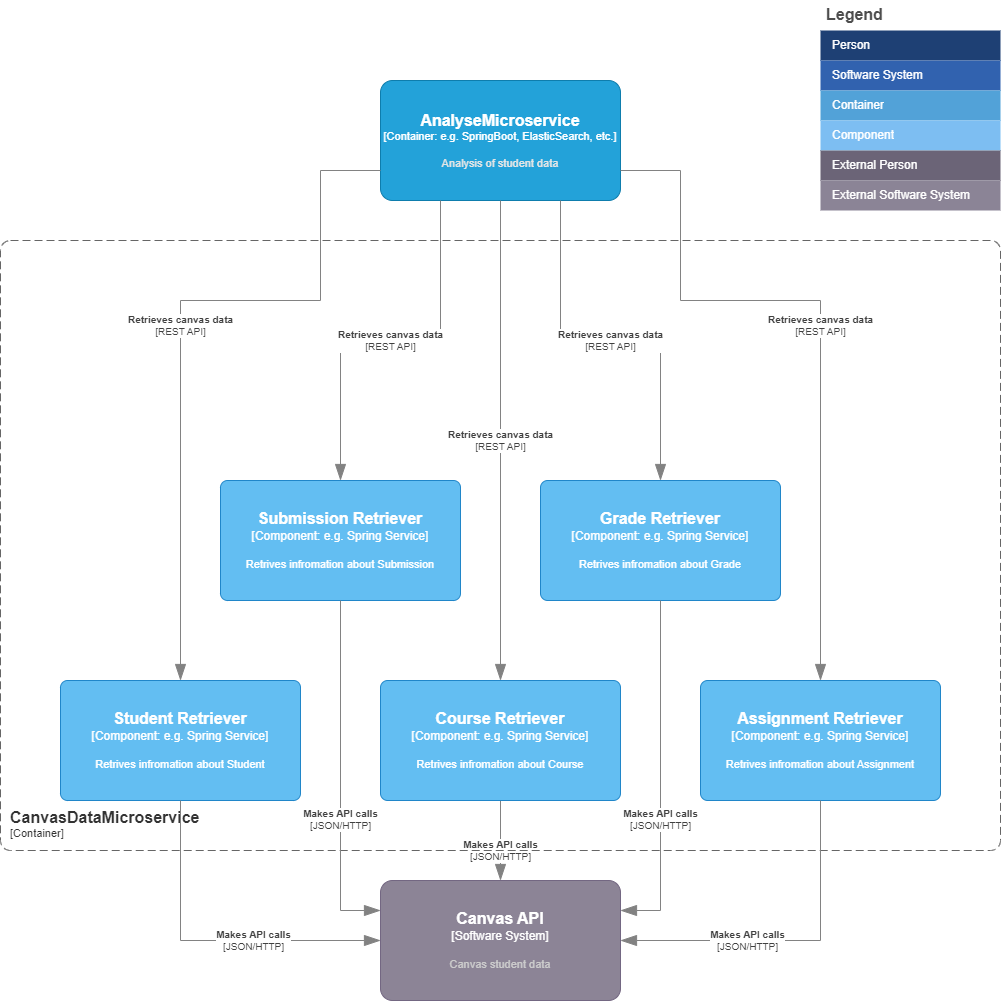
\includegraphics[width=\linewidth]{QSc4_3_CanvasDataMicroservice.png}
    \caption{Level 3 of C4 model}
    \label{fig:Level 3 of C4 model}
\end{figure}

\subsection{UML}
\begin{figure}[H]
    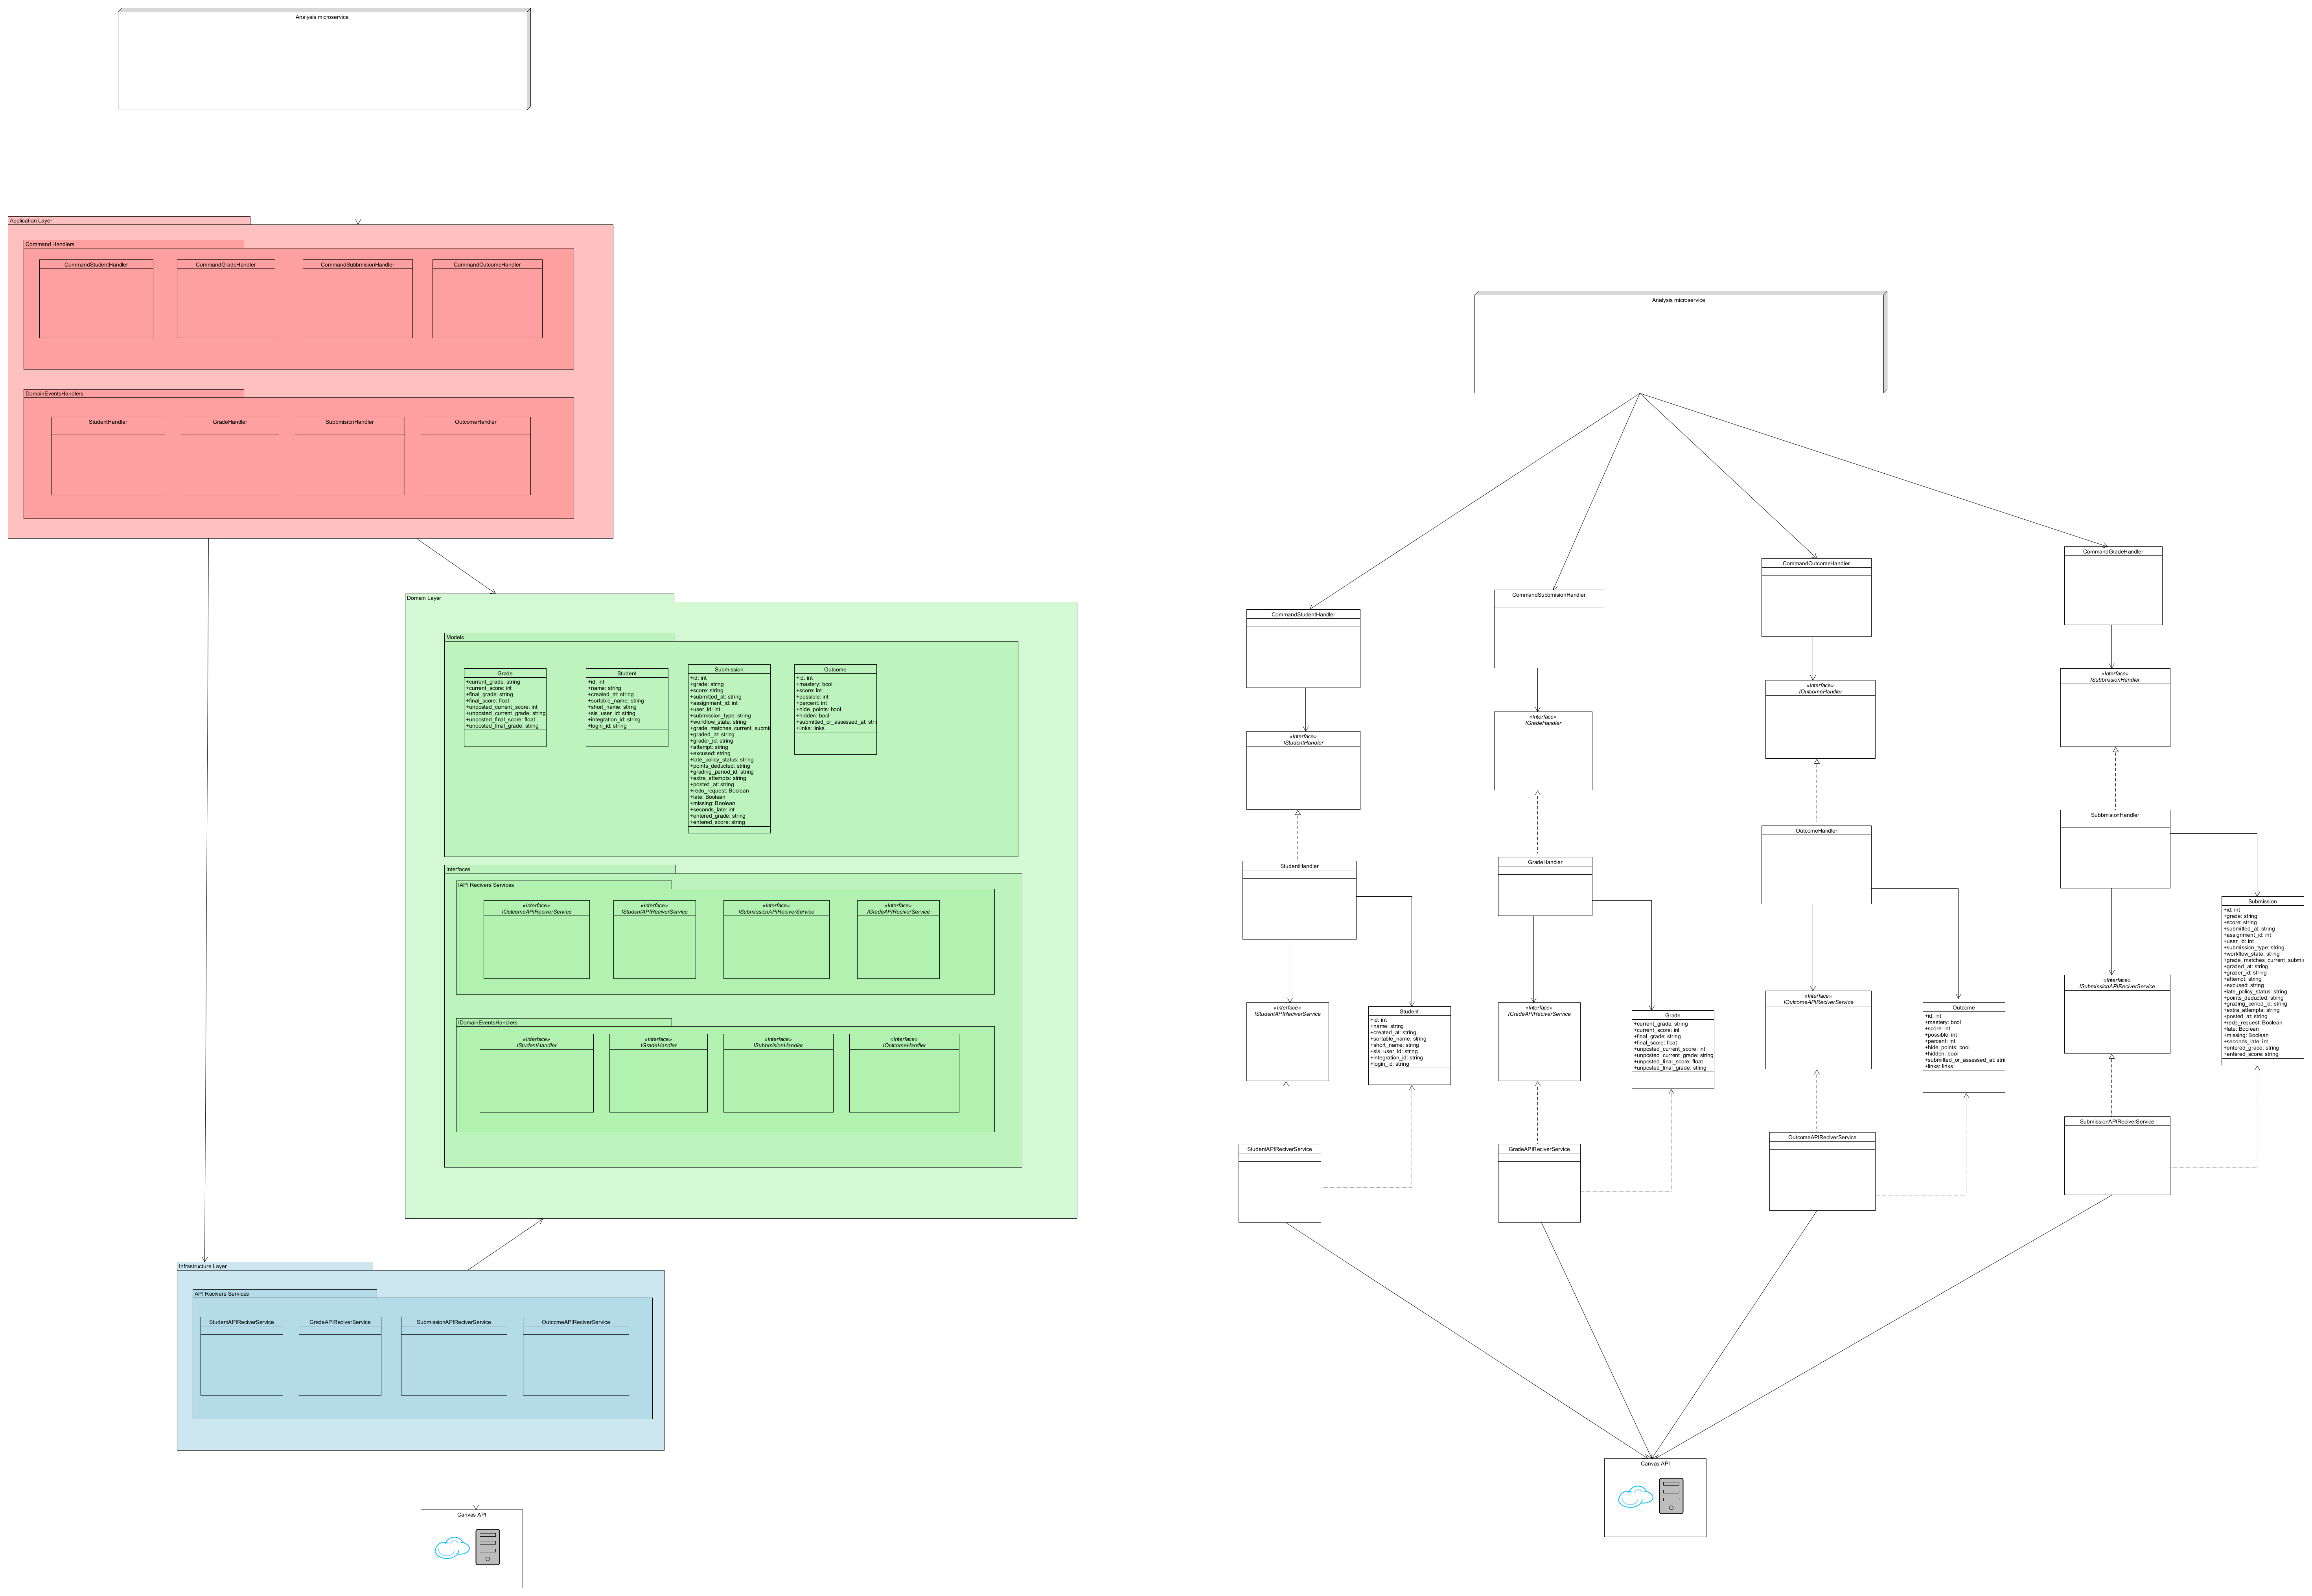
\includegraphics[width=\linewidth]{UML_CanvasDataMicroservice.png}
    \caption{UMLCanvasDataMicroservice}
    \label{fig:UML}
\end{figure}

\section{Data processing}
The Canvas Data Microservice plays a vital role in preparing and shaping data and objects for further usage within the Analyze Microservice and other components of the software. It acts as a data gathering and transformation layer, retrieving information on student scores, submissions, and grades from the Canvas learning management system. The microservice then processes and organizes this data, ensuring it is in a suitable format for analysis. It may perform data normalization, filtering, and aggregation, as well as handle any necessary data conversions. By preparing the data and objects, the Canvas Data Microservice enables seamless integration with the Analyze Microservice, allowing for efficient analysis and generation of insights. Additionally, other parts of the software can leverage the preprocessed data and objects for various purposes, such as generating reports, generating personalized recommendations, or powering visualizations in the web application dashboard. This way, the Canvas Data Microservice acts as a foundational component, providing the necessary groundwork for data-driven decision-making and enhancing the overall functionality of the software.

\section{Optimalisation}
During the development of the Canvas Data Microservice, optimization became a crucial focus due to prolonged data retrieval times. Recognizing the need to enhance performance, several measures were undertaken. Firstly, to address the slow data retrieval, specific data objects were trimmed down in size, retaining only the essential attributes required for analysis. By reducing the data payload, the microservice was able to retrieve and process information more efficiently, resulting in improved response times. 

Additionally, different API endpoints were devised to optimize data retrieval. This approach allowed for targeted requests, retrieving only the necessary data for analysis, further reducing latency and network overhead. Furthermore, to streamline the data retrieval process, REST API calls were modified to retrieve all the required data from a single Canvas API endpoint. This consolidation of data retrieval minimized the number of requests needed, significantly improving the overall efficiency of the microservice.

These optimization efforts, including data size reduction, the use of targeted API endpoints, and consolidating REST API calls, greatly improved the performance of the Canvas Data Microservice. By enhancing the speed and efficiency of data retrieval, the microservice ensures faster access to critical data for analysis, correlation, and presentation within the student performance dashboard.


\section{Conclusion}
In conclusion, the Canvas Data Microservice serves as a critical component in the software architecture, responsible for gathering, preparing, and organizing data and objects related to student scores, submissions, and grades. By leveraging domain-driven design principles, it ensures a cohesive and maintainable system structure. The microservice's role in preparing data for analysis within the Analyze Microservice and other parts of the software facilitates efficient processing, insightful analysis, and seamless integration. This enables data-driven decision-making, personalized recommendations, and the generation of meaningful insights to enhance educational outcomes. With its pivotal role in data preparation and object transformation, the Canvas Data Microservice plays a vital part in powering the software's functionality and supporting informed decision-making in the educational domain.




\pagebreak


\end{document}